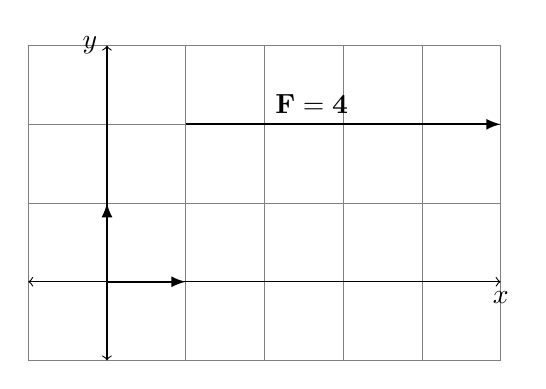
\begin{tikzpicture}
\centering

\draw[help lines] (-1,-1) grid (5,3);
\draw[thin, <->] (-1,0)--(5,0) node[below,black]{$x$};
\draw[thin, <->] (0,-1)--(0,3) node[left,black]{$y$};
\draw[thick,-latex] (0,0)--(1,0) node[below] {$\ax$};
\draw[thick,-latex] (0,0)--(0,1) node[left] {$\ay$};
%\node[below left](0,0){مرکز};
\draw[thick,-latex](1,2)--(5,2)node[pos=0.4,above] {$\bf{F}=4 \ax$};
\end{tikzpicture}%


